\documentclass[conference]{IEEEtran}
%\documentclass[11pt]{article} 
\usepackage[utf8]{inputenc} 
\usepackage[english]{babel}
\usepackage[T1]{fontenc}
%\usepackage{uarial}
%\renewcommand{\familydefault}{\sfdefault}
%\usepackage{blindtext}
%\renewcommand{\thepage}{\roman{page}}
%\usepackage{wordlike}
%\usepackage[tmargin=1in,bmargin=1in,lmargin=1in,rmargin=1in]{geometry}
\usepackage{geometry} % to change the page dimensions
\geometry{a4paper} % or letterpaper (US) or a5paper or....
\usepackage{graphicx} % support the \includegraphics command and options
\usepackage{verbatim} % adds environment for commenting out blocks of text & for better verbatim
\usepackage{amsmath}
%\usepackage{setspace}
\usepackage{amsfonts}
\usepackage{color}
\usepackage{listings}

\lstset{ %
language=FORTRAN,                % choose the language of the code
basicstyle=\footnotesize,       % the size of the fonts that are used for the code
numbers=left,                   % where to put the line-numbers
numberstyle=\footnotesize,      % the size of the fonts that are used for the line-numbers
stepnumber=1,                   % the step between two line-numbers. If it is 1 each line will be numbered
numbersep=5pt,                  % how far the line-numbers are from the code
backgroundcolor=\color{white},  % choose the background color. You must add \usepackage{color}
showspaces=false,               % show spaces adding particular underscores
showstringspaces=false,         % underline spaces within strings
showtabs=false,                 % show tabs within strings adding particular underscores
frame=single,           % adds a frame around the code
tabsize=2,          % sets default tabsize to 2 spaces
captionpos=b,           % sets the caption-position to bottom
breaklines=true,        % sets automatic line breaking
breakatwhitespace=false,    % sets if automatic breaks should only happen at whitespace
escapeinside={\%*}{*)}          % if you want to add a comment within your code
}
%\usepackage{sectsty}

%\doublespacing

\title{ParGA: A Parallelized Genetic Algorithm Framework in MATLAB}
\author{William McGinnis}

\begin{document}
\maketitle
%\clearpage
%\tableofcontents
%\clearpage
%\listoffigures
%\clearpage
%%%%%%%%%%%%%%%%%%%%%%%%%%%%%%%%%%%%%%%%%%%%%%%%%%%%%%%%%%%%%%%%%%%%%%
\begin{abstract}
Genetic Algorithms (GAs) are frequently used to find solutions to optimization and search problems. A GA finds solutions to these problems using techniques based on the concepts of natural evolution, namely mutation, inheritances and selection.  The mechanics of the algorithm itself lends it to parallelization, which can speed it up by large amounts, even on standard computers.  ParGA leverages the MATLAB parallel computing toolbox to parallelize a real-coded, single crossover GA.  It's modular design allows an objective function and fitness function to be simply plugged in.
\end{abstract}

\section{Framework}

ParGA is a MATLAB based framework for parallelized optimization problems.  It uses a real-coded genetic algorithm, in which the function calls for determining population fitness are parallelized.  The code is designed using the object oriented tools in MATLAB to allow for simple modification.  Exact usage is detailed in the Case Study presented later in the report.

The details of the algorithm itself pertain mostly to it's style of breeding, mutation, evolution and the parallelization itself.  

\subsection{Breeding}

The algorithm uses crossover breeding.  The user can select single, double, or no crossover (no crossover uses only mutation for variance).  In each breeding regardless of the crossover method used, the most fit half of the generation continues on unmodified into the next generation.  The 2nd half of the new generation is formed by using selected crossover breeding on random members of the last population, with those which are most fit being most likely to breed.

After this is done, the new generation is mutated at a user supplied rate and by a user supplied amount.  The mutation is performed with the following formula:

\begin{minipage}{0.43\textwidth}
\begin{lstlisting}
weights(index)=weights(index)*(((randn-1)/obj.kurt)+1); 
\end{lstlisting}
\end{minipage}

Where obj.kurt is the user supplied kurtosis value. The larger it is, the smaller the mutations will be. 

\subsection{Neighbourhooding}

Greater variation and the opportunity for multiple optima are accomplished by implementing neighbourhooding into the algorithm.  This means that N discrete, separate populations are evolved for some amount before being combined into one final population.  The amount of populations can be user selected, but care must be taken to ensure that the number of members per population is divisible by the number of neighbourhoods, otherwise there will be an error when merging the neighbourhoods. 

\subsection{Parallelization}

While the framework will run without error in serial, if the user has the MATLAB Parallel Computing Toolbox, then simply adding "matlabpool" into the run script, or typing it into the command window before running an optimization will let the code run in parallel.  This greatly speeds up the optimizations, especially when the fitness function is very computationally expensive.  

The code can also be run on more powerful machines such as clusters, with the configuration requirements depending on the cluster itself.  

Generally, the ideal number of cores to have is however many members per population you have, plus one for overhead.  Any more will not help very much if at all. 

\section{Case Study: Solid Rocket Motor Design}

In this case study, a solid rocket motor (SRM) legacy code was acquired from Dr. Hartfield, which was to be used to design a SRM to either have a specific thrust or chamber pressure output.  The desired output for thrust is a neutral 60,000 UNITS, and the desired output for chamber pressure is a neutral 500 UNITS.  

\subsection{FORTRAN Wrapper Function}

The legacy code was written in FORTRAN and used input and output files, which posed a small problem.  First and most importantly, input and output files cannot be used in the parallelized GA, because many nodes will be calling the function simultaneously, and the files cannot be read by multiple nodes simultaneously.  To solve this, the program was modified to run from command line.  

This is done in FORTRAN by using the IARGC() and GETARG() commands.  IARGC() returns the number of parameters passed through command line, and GETARG() returns those parameters.  Say, for instance, that you wanted to pass one variable, rpvar, to a program through command line.  To do this, you can use a code similar to the one below to get the arguments.

\begin{minipage}{0.43\textwidth}
\begin{lstlisting}
        integer :: jcount
        real :: jtemp
        character(len=32) :: arg
        
        jcount=IARGC()
        if (jcount==1) then
           call GETARG(1,arg)
           read(arg,*)jtemp
           rpvar=DBLE(jtemp)
        end if
\end{lstlisting}
\end{minipage}

The variable, rpvar, can then be used to compute some kind of fitness (to be minimized), and the fitness is printed to command line with the code:

\begin{minipage}{0.43\textwidth}
\begin{lstlisting}
	print*, "", fitness
\end{lstlisting}
\end{minipage}

This will write the value stored in the variable, fitness, to the command line, where it can be read by another program.  

\subsection{MATLAB Integration}

In the case of the SRM code, the FORTRAN wrapper function takes in 8 variables, uses them to calculate a thrust or chamber pressure profile, and returns the percent RMS error.  In both cases, the RMS error is to be minimized, with a goal of under 1\%.  As with any optimization problem solved with ParGA, the first step is to write the fitness function.   This function should contain all code to calculate the fitness of the Member, given the gene.  The general form of a fitness function is:

\begin{minipage}{0.43\textwidth}
\begin{lstlisting}
function out=sample_fn(gene)
 %calculate fitness using gene and set out equal to it
\end{lstlisting}
\end{minipage}

The entire fitness function in this case study is:

\begin{minipage}{0.43\textwidth}
\begin{lstlisting}
function out=sample_fn(gene)
command=sprintf('SRM_serve.exe %20.10fd0 %20.10fd0 %20.10fd0 %20.10fd0 %20.10fd0 %20.10fd0 %20.10fd0 %20.10fd0', gene);
[~,result]=system(command);
out=str2double(result);
\end{lstlisting}
\end{minipage}

Next, the run script is written to actually build and perform the algorithm.

\begin{minipage}{0.43\textwidth}
\begin{lstlisting}
close all; clear all;clc;

mins=[0.01,0.01,.1,0.01,
	0.01,0.01,0.1,0.01];
maxes=[0.95,0.99,13,0.2,
	0.999999,0.77,100,0.667];
rate=0.08;
kurt=10;
crossover=0;

gen_sample1=Globe(@sample_fn,4,1000,64,mins,maxes,kurt,rate,crossover);

gen_sample2=gen_sample1.evolveCommunities;

gen_sample3=gen_sample2.mergeCommunities;

gen_sample4=gen_sample3.evolveGlobe;
\end{lstlisting}
\end{minipage}

This will create an optimization with 4 neighborhoods, 1000 generations per epoch, 64 members per population, a mutation rate of 8\%, and a kurtosis parameter of 10.  No crossover will be used, so mutation will be the sole mode of variation.  Line 14 evolves the 4 separate neighborhoods 1000 generations each.  Line 16 takes the best quarter of each neighborhood and combines them into one population.  Finally, line 18 evolves the combined population for 1000 generations.  The final population can be evolved again as many times as desired by calling gen\_sample4.evolveGlobe again. 

Once this is completed, the final solution can be printed with the code:

\begin{minipage}{0.43\textwidth}
\begin{lstlisting}
popfitness=gen_sample4.nations.popfitness;
[empty,ix]=sort(popfitness);
gene=gen_sample4.nations.pop{1,ix(1)}.gene;
command=sprintf('SRM_serve_print.exe %20.10fd0 %20.10fd0 %20.10fd0 %20.10fd0 %20.10fd0 %20.10fd0 %20.10fd0 %20.10fd0',gene);
[~,result]=system(command);
plot_data=sscanf(result,'%f\t');

figure;
plot(plot_data);
ylabel('Thrust');
title('Neutral Thrust Result')
\end{lstlisting}
\end{minipage}

Where the program, SRM\_serve\_print.exe, returns the entire thrust time series.

\subsection{Results}

The optimization was run on a quad core desktop computer with the parameters described in the previous section, for thrust.  This amounts to a total of 40,000 function calls, which when parallelized is equivalent to 10,000 function calls in serial.  The resultant RMS error percentage was 0.0001277538\%, which was far better than the goal of 1\%.  The gene which resulted in this error was:

\begin{align}\notag
rpvar\ &=\ 0.5519\\\notag
 rivar\ &=\ 0.3042\\\notag 
 xnx\ &=\ 2.1415\\\notag
 fvar\ &=\ 0.0867\\\notag
  epsx\ &=\ 0.0940\\\notag
fnlx\ &=\ 0.0314\\\notag
glx\ &=\ 21.3500\\\notag
 diathx\ &=\ 0.6670\notag
 \end{align}

And the resultant thrust profile is shown in Figure \ref{fig:thrust}.

\begin{figure}[h!t]
 \centering
    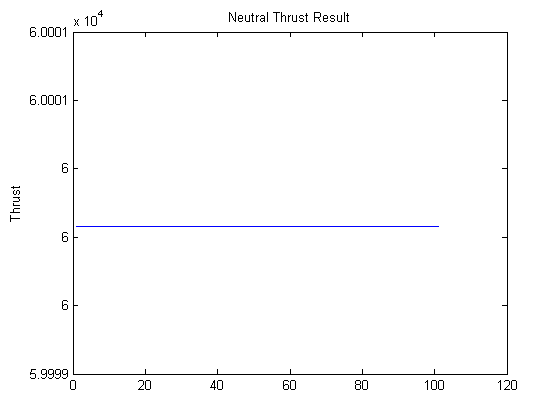
\includegraphics[width=3in]{thrust.PNG}
    \caption{Thrust Profile of Optimal Solution}
    \label{fig:thrust}
\end{figure}


This result was found in 819.71 seconds.  This amounts to a 1.84x speedup over the time to run in serial of 1514.24 seconds. 

\section{Code}

All of the code for this toolbox can be found at:

https://github.com/wdm0006/ParGA
%\bibliography{bibtex_database} 
%\bibliographystyle{plain}

\end{document}




















